%*****************************************
\chapter{La perception de l'environnement sonore}\label{ch:psycho_ea}
%*****************************************

Avant d'aller plus loin dans la présentation de nos recherches, ils nous est indispensable ici de dresser un état des lieux des connaissances liées à la perception des sons.

Nous proposons de présenter ces connaissances en quatre parties. La première récapitule les processus de traitement connus et mises en œuvre à partir du moment où le signal atteint le récepteur, autrement dit le tympan. 

Dans un second temps, nous présentons les résultats émanant de différentes études, regroupées a posteriori sous l'appellation Analyse de Scènes Acoustiques (ASA), et qui s'intéressent à la manière dont le cerveau assimile/ségrègue  les différentes informations contenues dans l'environnement sonore afin d'en dégager des objets cohérents, \ie des sources sonores. 

La troisième partie présente quant à elle les résultats d'études s'attachant a comprendre le fonctionnement  des mécanismes haut niveaux opérant lors de l'évaluation perceptive des environnements sonores, en empruntant une méthodologie issue de la psychologie cognitive. Il s'agit en particulier, d'étudier la contribution, sur l'évaluation globale, des objets composant ces environnements.

Enfin, la dernière partie résume, de manière non exhaustives, ce que le domaine des neurosciences nous apprend sur le traitement de l'information sonore par le cerveau. 

\section{Étudier le traitement de l'information auditive}

\subsection{Perception et cognition}

La perception désigne l'ensemble des processus de traitement de l'information sensorielle. Ces processus nous permettent, par l'interprétation des données reçues en continu par nos organes, de construire une représentation interne du monde qui nous entoure [p. ??]\citep{Houix03f}.

La perception du monde sonore qui nous entoure est un phénomène complexe et encore mal connu. Cette perception est à l'origine de l'interaction que nous créons avec notre environnement. Elle détermine notre capacité d'adaptation à ce dernier. Cette relation au monde \emph{réel} ne se rompt jamais. Nous percevons des sons en permanence, et ce, même si aucune source sonore n'est présente. Ainsi, à la seule lecture d'une partition de musique, le musicien entraînée est capable d'entendre la musique comme si elle était jouée.

Pour la cognition, nous partons d'une définition proposée par U. Neisser \footnote{Ulric Neisser est considéré comme un des pères du cognitivisme notamment grâce à son livre \citep{neisser1967cognitive}. Il a par la suite beaucoup critiqué la direction prise par le mouvement, lui reprochant son recourt excessif aux travaux en laboratoire au détriment des conditions in situ.} dans \citep[p. ??]{neisser1976cognition} .

\begin{quote}
Cognition is the activity of knowing : the acquisition, organisation and use of knowledge.
\end{quote}

Le terme cognition renvoie à la notion de connaissance. Dans un sens plus précis, il désigne les conditions qui permettent l'acquisition et le développement d'une connaissance du monde.

Selon la théorie classique, perception et cognition dépendent de deux groupes de systèmes fonctionnels du cerveau distincts. La perception mobilise les systèmes de traitement dits modaux, c'est à dire supportés par les organes sensoriels (oreilles, yeux etc $\ldots$), tandis que les systèmes cognitifs s'appuient sur des représentations mentales des réalités externes, par essence amodales.

Cette dichotomie entre perception et cognition a été plus récemment critiquée. Dans une approche ``\,incarnée\,'' de la cognition (\emph{Grounded Cognition}), Barsalou nie le caractère amodal des représentations mentales prônant que ces dernières dépendent également des modalités sensorielles \citep{barsalou2010grounded}. Il tente ainsi de réunir les processus perceptifs et cognitifs \citep{goldstone1998reuniting, barsalou1999perceptions}. 

Les deux approches sont illustrées sur la Figure~\ref{fig:processusPercepAndCo}.

\begin{figure}[bth]
        \myfloatalign
        \includegraphics[width=.6\linewidth]{gfx/Representation}
        \caption{Processus cognitifs et perceptifs}\label{fig:processusPercepAndCo}
\end{figure}


\subsubsection{Psychologie cognitive et psychoacoustique}

La psychologie cognitive est un domaine de recherche dédié aux phénomènes se rapportant à la connaissance. Elle est née dans les années 50, en réaction au \emph{Béhaviorisme}, théorie qui se fonde sur ``\,l'étude des comportements objectivement observables de l'être humain\,'', négligeant, de fait, le rôle de la conscience. La psychologie cognitive, au contraire elle, s'interroge sur des modèles théoriques complexes rendant compte de tous les faits et de toutes les lois connus. Les chercheurs y explorent tout à la fois, la mémoire, le langage, l'intelligence, la perception

L'approche cognitiviste, dans l'étude de la perception auditive, s'éloigne de celle plus traditionnelle de la psychoacoustique \footnote{La psychoacoustique est une branche de la psychophysique qui applique au domaine de l'acoustique les concepts et les méthodes ayant cours en psychophysique.}. Tandis que la psychoacoustique émet l'hypothèse d'une relation directe entre un stimulus et la réponse de l'individu à ce dernier, la psychologie cognitive soutient qu'à un stimulus, l'homme donne des réponses entièrement corrélées au contexte, à l'expérience, aux interactions multi-sensorielles \citep{maffiolo_marieParis_1997}. Ces réponses tiennent compte non seulement des traitements perceptifs mais aussi des représentations issues et de la mémoire individuelle (\ie~construites en particulier à partir de la relation sensible au monde) et de la mémoire collective, à travers le développement des connaissances partagées \citep[p. ??]{maffiolo_caracterisation_1999}.

La psychologie cognitive s'intéresse prioritairement à l'aspect cognitif de la perception en considérant l'individu comme un tout. Elle prend en compte la culture, l'expérience, l'activité de l'individu et ne se focalise pas seulement sur la réaction des organes sensoriels comme l'oreille. Elle questionne les aspects qualitatifs plus que quantitatifs de notre compréhension du monde sonore \citep[p. ??]{maffiolo_caracterisation_1999}.

Elle envisage l'ensemble des étapes du traitement auditif de manière globale et permet ainsi de faire le lien entre une information sensorielle et une information abstraite \citep{mcadams1994penser}.

\subsubsection{Paradigme de la psychologie cognitive}

Comme nous l'avons vu, le cognitivisme ne conçoit pas l'individu comme une ``\,boîte noire\,'', mais envisage ce dernier comme un système de traitement de l'information. Le cognitivisme, fait ainsi l'analogie entre le fonctionnement humain et le fonctionnement de l'ordinateur.

Il ne défend pas l'hypothèse d'un comportement linéaire entre un stimulus externe et la réponse du sujet. Il admet au contraire que le sujet adopte une stratégie, dans le but d'optimiser son comportement face au stimulus. Cette stratégie dépend de la nature du stimulus, du contexte ainsi que des connaissances a priori du sujet.

Maffiolo propose un résumé des présupposés sur lesquels repose le cognitivisme, et qui sont résumés sur la Figure~\ref{fig:paradigmeCognitivisme} \citep[p. ??]{maffiolo_caracterisation_1999} :

\begin{itemize}
\item le monde est discrétisé en dimensions ou propriétés issues de la physique, considérées comme vraies
\item ces dimensions ou propriétés peuvent être mesurées objectivement par des instruments, rendant ainsi compte de la réalité
\item le sujet intègre de manière séquentielle ces dimensions ou propriétés en fonction du contexte
\item l'évaluation subjective du sujet est mesurée comme un décalage par rapport à la mesure objective considérée comme vraie
\end{itemize}

Au regard du paradigme classique de la psychologie cognitive, Maffiolo met en évidence quatre points discutables :

\begin{itemize}
\item la pertinence des dimensions et propriétés physiques utilisées pour le découpage du monde
\item un traitement par les sujets tenant spécifiquement compte de ces dimensions
\item une séparation nette entre stimulus et contexte
\item le caractère subjectif du jugement humain en comparaison à l'objectivité d'un appareil de mesure.
\end{itemize}

\begin{figure}[bth]
        \myfloatalign
        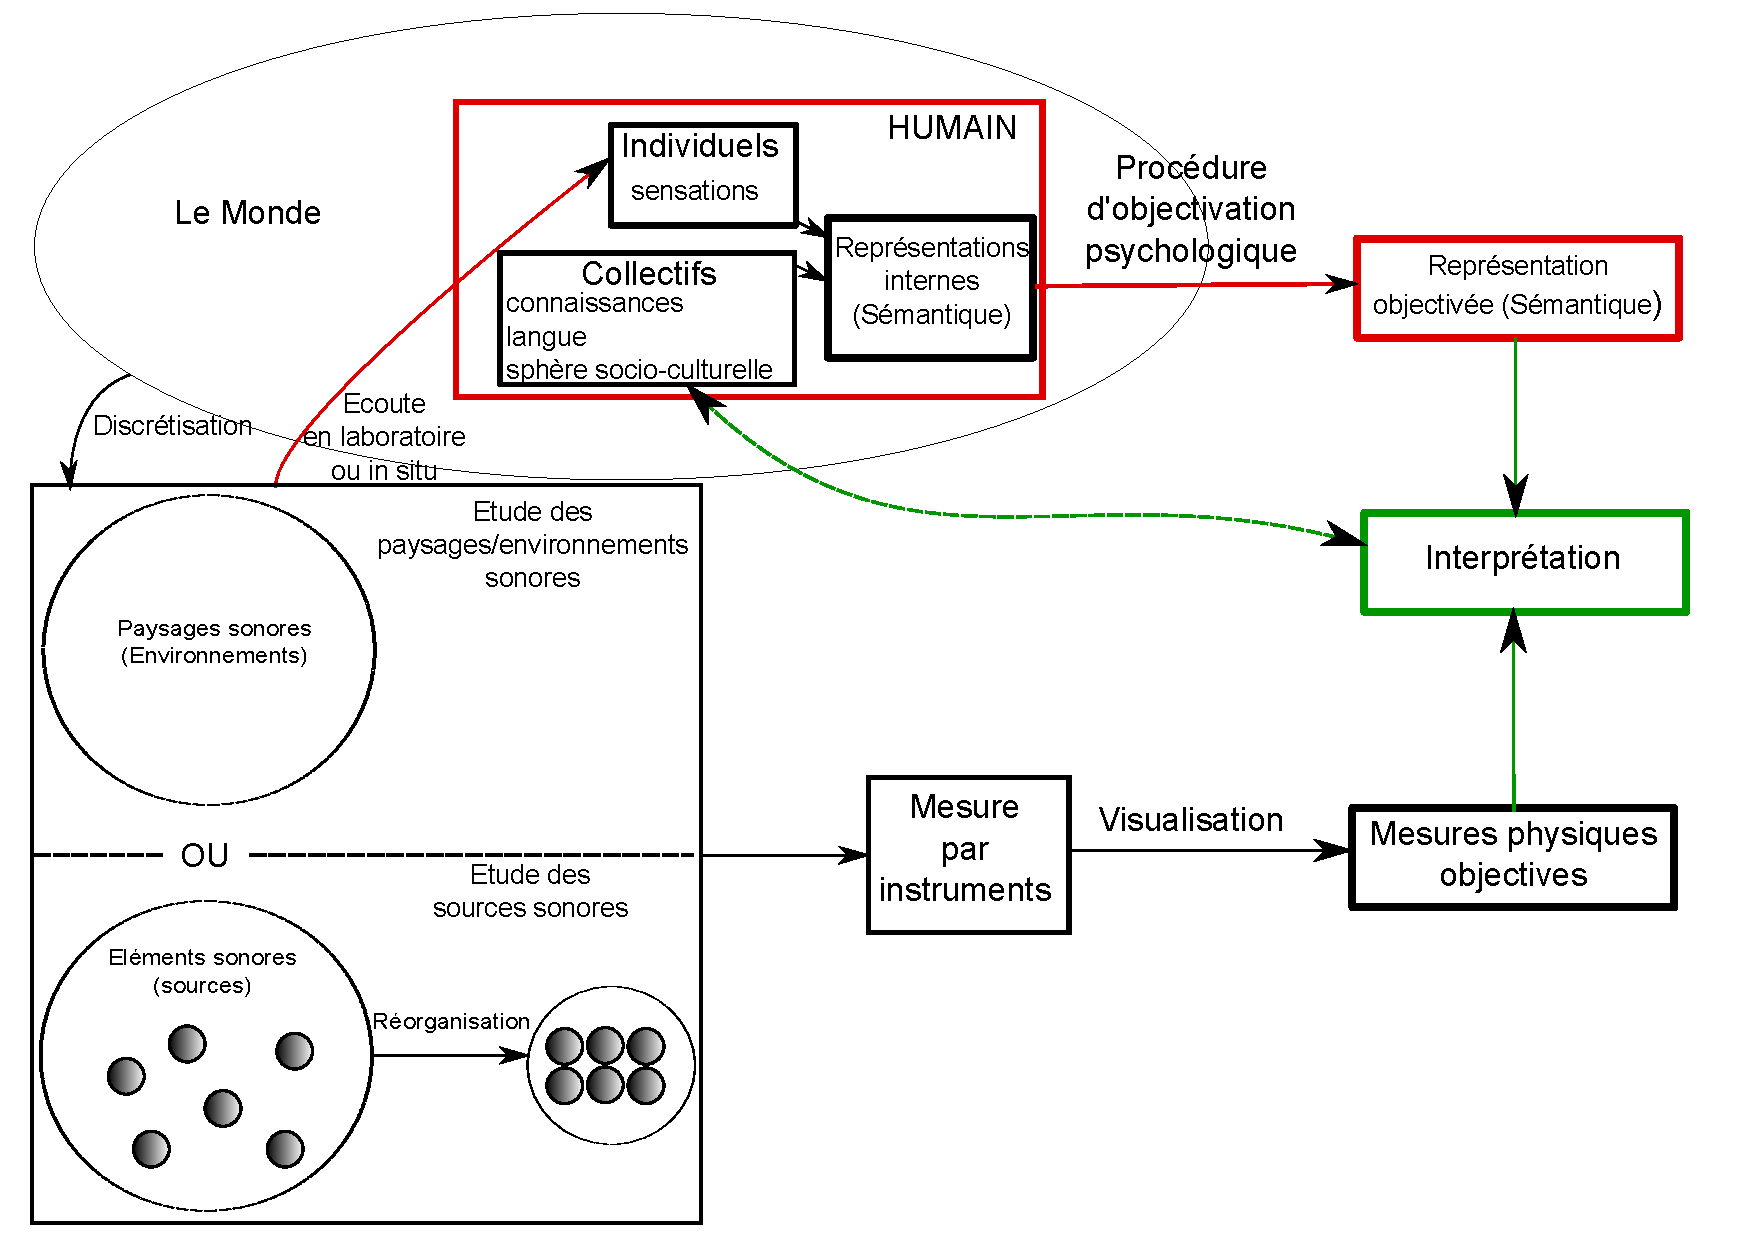
\includegraphics[width=.9\linewidth]{gfx/Shema_maffiolo}
        \caption[Paradigme du cognitivisme]{Paradigme du cognitivisme, d'après \citep{maffiolo_caracterisation_1999}}\label{fig:paradigmeCognitivisme}
\end{figure}

\subsubsection{L'approche Écologique}
\label{sec:ecologique}

L'approche écologique a d'abord été introduite dans le domaine de la vision par Gibson \citep{gibson1966senses}, qui se demande entre autre si les ``\,lois structurant les objets sont porteuses d'informations, ou si cette information est tirée de comparaison\,'' \citep{gibson1978ecological}.

Cette approche reconnaît que la réponse à un stimulus dépend et de l'information perçue (processus \emph{bottom-up}), et de la connaissance du monde (processus \emph{top-down}), autrement dit l'environnement quotidien et le contexte habituel d'écoute du stimulus.


\subsection{Le chaîne traitement de l'information auditive}
\label{sec:chaineTaite}

Le son est une vibration émise par une source d'excitation, et transmise à l'air. Cette vibration se propage ensuite jusqu'à atteindre un récepteur, le tympan, qui va capter le différentielle de pression résultant de cette vibration. C'est le point de départ du processus de traitement de l'information auditive. 

Si on adopte une approche \emph{traitement de l'information}, on peut décomposer ce processus en plusieurs systèmes inter-connectés. Ces systèmes forment une chaîne qui, au fur et à mesure des traitements, interprète le signal acoustique afin d'en extraire information sémantique. Plus on se place loin dans la chaîne de traitement, plus on a accès à une information abstraite, potentiellement utilisable par d'autres processus de haut niveau. La figure \ref{fig:traitementSonMcAdamsBigand} extraite de \citep{mcadams1994penser} nous donne un aperçu des principales fonctionnalités du système de traitement auditif.

\begin{figure}[bth]
        \myfloatalign
        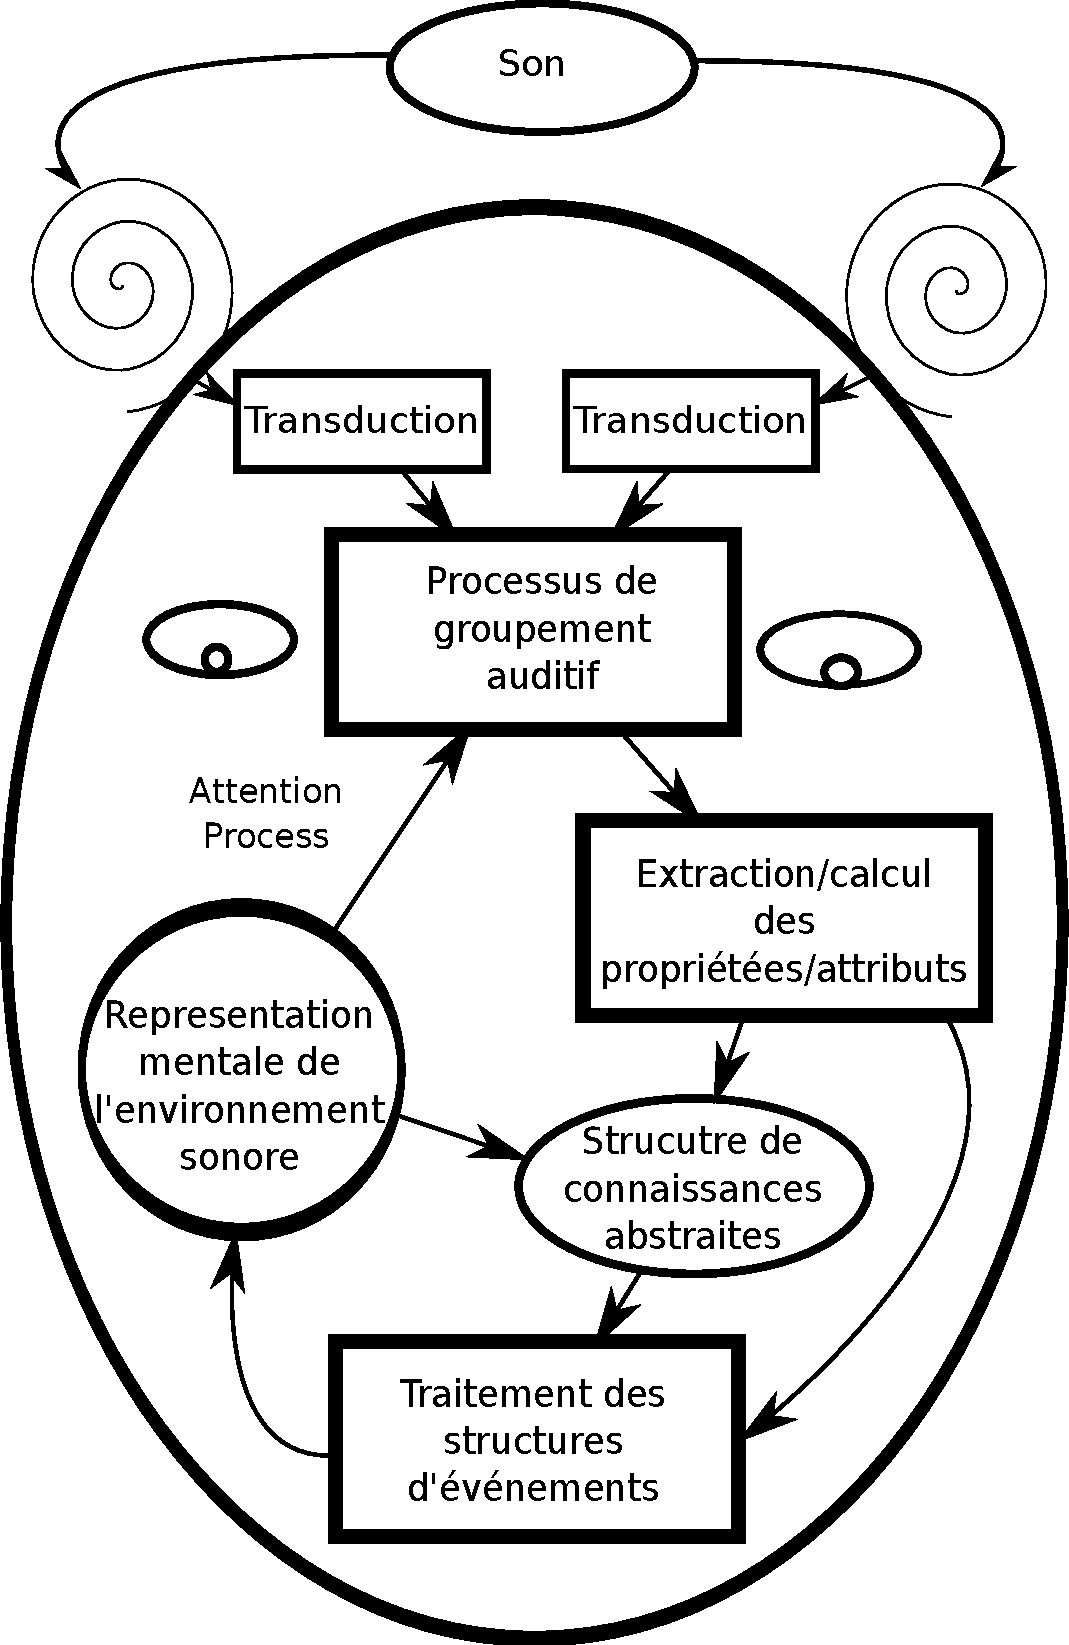
\includegraphics[width=.5\linewidth]{gfx/traitementSonMcAdamsBigand}
        \caption[Principaux processus de traitement de l'information auditive et leurs interactions]{Principaux processus de traitement de l'information auditive et leurs interactions, à partir de \citep{mcadams1994penser}}\label{fig:traitementSonMcAdamsBigand}
\end{figure}

Lors de l'étape de \emph{transduction}, les vibrations sonores parvenant au tympan sont analysées puis traduites en impulsions nerveuses transmises au cerveau. Ces impulsions rendent compte des attributs spectraux et temporels de l'onde. L'extraction des composantes fréquentielles intervient dans la cochlée, dans laquelle différentes parties de la membrane basilaire vont être excitées en fonction des fréquences composant le signal, suivant un axe tonotopique. Les vibrations captées à chaque point d’excitation de la membrane basilaire sont transmises au cerveau via les nerfs auditifs, chaque point codant une information correspondant à une bande fréquentielle limitée. 

Vient ensuite le \emph{processus de groupement auditif}. C'est une étape d'intégration temporelle au cours de laquelle l'information est analysée en images auditives cohérentes. Contrairement à ce que pensaient les Grecs, nous ne possédons pas de "canaux" séparés pour chaque objet sonore présent dans l'environnement \citep{yost1994fundamentals}. C'est notre cerveau qui se charge de fusionner et de discrétiser les éléments sonores simultanés afin de créer un flux auditif structuré. En d'autres termes il s'agit de déterminer, combien d'objets sonores sont présents, d'où viennent t-ils et quel est leur sens. Les recherches regroupées sous l'appellation ``\,analyse de scènes auditives\,'', abordées à la section~\ref{sec:ASA} ont  extensivement étudié ces processus de groupement.

Prenons pour exemple les chorals de Bach. C'est le \emph{processus de groupement auditif} qui nous permet, sur la base des paramètres spectro-temporels du signal, de distinguer les quatre voix basse, ténor, alto et soprano. Par contre c'est à partir d'une analyse des attributs perceptifs que nous sommes capables de percevoir les mélodies comme des objets unitaires, même si ces dernières sont développées entre les différentes voix du choral. Cette extraction des propriétés perceptives intervient pendant la phase dite \emph{d'extraction/calcul des propriétés/attributs}.

Une définition des représentations mentales est donnée par \citep{houde1998vocabulaire}:

\begin{quote}
``\,La représentation mentale peut être vue comme une entité interne, le correspondant cognitif individuel des réalités externes expérimentées par un sujet.\,''
\end{quote}

Ces représentations font office de sauvegardes de l'information. Conservées en mémoire sous une forme hautement abstraite \citep[p. ??]{mcadams1994penser}, elles rendent compte à la fois de notre compréhension du monde et de la manière dont nous l'abordons. Ces connaissances subjectives, non directement observables, restent néanmoins accessibles au chercheur par le biais d'expériences d'objectivation.

\subsection{Processus Bottum-up et processus Top-down}


L'interaction entre l'homme et son environnement est fonction d'une part de l'information sensorielle captée par le sujet, d'autre part de la rétroaction exercée par lui sur ces données. Cette rétroaction est déterminée par son expérience sensible du monde. Par "expérience sensible", nous entendons la mémoire interne des interactions passées, mémoire grâce à laquelle nous optimisons l'analyse des stimuli, et intégrons les effets de contexte dus à l'environnement.

Cette mémoire est à la fois :

\begin{itemize}
\item individuelle : dépendant de notre expérience propre
\item collective : dépendant des connaissances que nous avons acquises sur le monde
\end{itemize}

La rétroaction est l'expression de l'individualité du sujet, individualité qui explique que deux personnes ayant des capacités sensorielles semblables peuvent percevoir différemment un même environnement.

Ainsi la perception mobilise deux formes de traitements :

\begin{itemize}
\item les traitements dits ascendants (bottom-up) dirigés par les données
\item les traitements dits descendants (top-down) dirigés par les concepts ou les représentations
\end{itemize}

Étudier la perception demande de prendre en compte aussi bien l'information externe (processus ascendant) que l'information interne (processus descendant). Réduire la perception à une simple association de sensations ne permet pas de rendre compte de l'éventail des processus cognitifs entrant dans le décodage de l'environnement. Un exemple parlant concret, emprunté au domaine de la vision, est celui du phénomène dit de bi-stabilité, \ie~La faculté, chez un sujet, de voir dans une même image tantôt un canard, tantôt un lapin, autrement dit, de tirer d'un même stimulus deux analyses différentes, mais jamais simultanément (Cf. Figure\ref{fig:bistabilite}).

Un autre exemple, cette fois dans le domaine de l'audition, nous semble illustrer le caractère dual de la perception. Il est donné par McAdams et Bigand \citep[p. 2]{mcadams1994penser}:

\begin{quote}
``\,...Imaginez vous un instant en pleine forêt amazonienne : vous entendriez exactement les mêmes bruits que le guide qui vous accompagne, mais, étant donné votre manque de connaissance du milieu, vous seriez incapable d'extraire du fond sonore les sons correspondant aux cris de l'iguane, aux singes macaques, aux chants des ouistitis ou aux bruissements des arbres tropicaux. De ce fait vous seriez dans l'incapacité d'attribuer une signification à l'ensemble de la structure sonore, ce qui pourrait être important pour votre survie dans l'environnement.\,''
\end{quote}

\begin{figure}[bth]
        \myfloatalign
        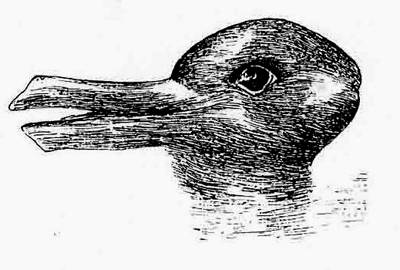
\includegraphics[width=.5\linewidth]{gfx/canard_lapin}
        \caption{Un exemple du phénomène de bi-stabilité}\label{fig:bistabilite}
\end{figure}

En psychologie cognitive, on distingue ainsi les approches cognitivistes, qui s'intéressent plus particulièrement aux processus de type \emph{botttom-up} relatifs au traitement de l'information perçue , des approches dites cognitives, lesquelles interrogent, avant tout, les processus de type \emph{top-down} liés à la mémoire du sujet ainsi qu'au contexte \citep[p. ??]{guastavino_etude_2003}.

\section{Analyse de scènes acoustiques}
\label{sec:ASA}

\subsection{Introduction}

L'analyse de scène est un terme d'abord introduit de la cadre des recherches informatiques en vision. Il fait référence aux différentes stratégies par laquelle un ordinateur parvient à isoler un objet du image~\citep[p. 12]{mcadams1994penser}. Le pendant acoustique de l'analyse scène, est nommé l'Analyse de Scène Acoustique (ASA). Le terme ASA a été introduit par Albert S. Bregman dans son ouvrage de référence \citep{bregman1994auditory}.  

L'ASA désigne l'ensemble des processus perceptifs permettant d'isoler dans  mixture sonore \footnote{On entend par mixture sonore, ou magma sonore, un ensemble de sons provenant de différentes sources sonores}, les informations émanant des mêmes sources sonores, et à les regrouper afin de les traiter comme un tout cohérent.  L'ASA part en effet du principe que, afin de faire sens de l'environnement qui l'entour, il est nécessaire pour le cerveau d'isoler les informations relatives aux différentes sources sonores \citep{winkler2009modeling}. On parle alors indifféremment de processus de ségrégation ou de groupement.

La définition de l'ASA est très large. En effet, comme vu dans la section~\ref{sec:chaineTaite}, les processus de groupement sont composés à la fois de processus \emph{bottum-up}, \ie~ dirigés par l'information auditive transduite (représentation temps-fréquence du signal sonore), ainsi que de processus \emph{top-down} dirigés par les connaissances stockées en mémoire. Dans la théorie de l'ASA, les processus \emph{bottum-up} sont appelés \emph{processus primitifs}, et les processus  \emph{top-down}, \emph{processus basés sur des schémas}. Pour les premiers, il s'agit de systèmes de traitement innés, opérant sur la base de régularités présentes dans le signal, afin de regrouper les composantes fréquentielles produites par une même source. Par régularité on comprend ici des propriétés constantes de l'environnement, perçues par l'ensemble des êtres humains, partout sur la planète. Par exemple, si la fréquence fondamentale d'un son harmonique change au cours du temps, toutes ses harmoniques changeront également afin de maintenir la structure harmonique du son [p. 38]\citep{bregman1994auditory}. Les \emph{processus basés sur des schémas}  partent eux de schémas (\ie~connaissances apprises formant notre représentation mentale du monde), formés par le biais d'écoutes antérieures. 

L'acceptation de l'existence de ces deux approche montre que l'ASA s'inscrit bien dans une vision cognitive de l'audition. Cependant, la plupart des études se sont concentrés sur les \emph{processus primitifs}, en adoptant un approche méthodologique très inspirée de la psychoacoustique.


\subsection{Une approche psychoacoustique}

L'étude de l'ASA adopte une méthodologie s'inspirant largement du paradigme de la psychoacoustique. Ainsi les réponses du sujets sont évaluées par rapport à un stimuli décrit analytiquement dans un espace multidimensionnel de dimensions physiques (fréquence, intensité etc $\ldots$) \citep{dubois2006cognitive}. Dans la grande majorité des cas, les stimuli utilisés sont des sons pures ou complexes\footnote{Par son pur on entend un son composé d'une seule sinusoïde, \ie~possédant une seule fréquence. A contrario, un son complexe est un son composé de plusieurs composantes fréquentielles}, bien évidemment synthétisés en laboratoire. 

Ces sons sont alors proposés à l'écoute à un sujet, et ce de manière séquentielle. Il s'agit alors, au cours de la séquence, de faire varier un paramètre (intensité, hauteur fréquentielle, espacement entre les séquences), et d'observer le seuil à partir duquel ce changement a un effet significatif sur la capacité du sujet à distinguer plusieurs sources sonores.

L'étude de l'ASA se restreint donc à l'analyse de l'effet de descripteurs bas niveaux sur les processus d'intégrations, sans tenir compte d'attributs perceptifs plus haut niveaux, comme la valeur sémantique attribuée aux sons, ni de considérations écologiques~\ref{sec:ecologique}. En conséquence, il est parfois difficile de faire le lien entre la notion de source sonore comme utilisée dans les études psychoacoustique de l'ASA, et celle adoptée par les études en psychologie cognitive. En théorie, pour les deux approches, le terme source sonore se réfère directement à l'objet (\eg~voiture) supposé être la source d'émission d'un son réel. En psychologie cognitive, cette relation est directe, le stimuli étant la plupart du temps un enregistrement de ladite source. En psychoacoustique, la relation directe est difficile, les stimuli étant des sons de synthèses, inexistant dans le monde réel. La source sonore désigne alors plutôt un objet abstrait, dont l’existence est avérée à partir du moment ou un agglomérat de sinusoïdes est interprété par le sujet comme étant un tout, émanant de facto d'une seule entité. 

Il s'agit là d'une des limitations de l'approche psychoacoustique appliquées aux études des processus primitifs de l'ASA. Les résultats, obtenus à partir de stimuli très éloignés de la réalité des phénomènes acoustiques perçus, étant difficiles à généraliser à des cas d'études plus incarnés.

\subsection{Gestalt Theory}

L'ASA a permis de montrer que la perception des sons suit, en grande partie, les mêmes règles que celles observés pour la vision, et notamment les principes décrits par la \textit{Gestalt Theory}.

\subsection{Le Streaming}

\subsection{Processus de ségrégation}

\subsection{L'approche par les neurosciences}


\section{Le paysage sonore}
\label{sec:psychoCog}

\subsection{Introduction}

\subsubsection{La notion de paysage sonore}

La notion de paysage sonore a été introduite par Schafer dans les années soixante-dix
dans son livre \citep{schafer1969new} et détaillée dans l'ouvrage de référence \citep{schafer1977tuning}. La question que se pose Schafer est alors:

\begin{quote}
Quelle est la relation entre l'homme et les sons de l'environnement qui est le sien, et que se produit-il lorsque ces sons viennent à changer ?
\end{quote}

Bien qu'il n'existe pas de définition consensuelle d'un paysage sonore, la communauté de recherche semble s'accorder \cite{niessen2010categories} sur celle donnée par B. Truax \citep{truax1978handbook}:

\begin{quote}
Un environnement sonore tel qu'il est perçu et compris par un individu ou une société.
\end{quote}

La définition se veut très générale. Tout environnement peut être considéré comme un paysage sonore si tant est qu'on lui associe un ensemble de son entendus par un sujet donné. Le point capital est d'envisagé l’environnement sonore par rapport à l'évaluation subjective de l'auditeur, plutôt que de ne prendre en compte que ses paramètres acoustiques.

Ainsi, les études sur les paysages sonores suivent le paradigme de la psychologie cognitive \citep{dubois2006cognitive,maffiolo_caracterisation_1999} (voir~\ref{sec:psychoCog}). L'environnement sonore est décrit en utilisant à la fois des descripteurs acoustiques (mesures), ainsi que des descripteurs perceptifs, l'analyse de l'interaction entre ces descripteurs permettant de comprendre les processus cognitifs mis en œuvre dans l'évaluation perceptive des paysages sonores.

Schafer explicite la nécessité de ne plus considérer seulement le bruit, mais également sa perception par les individus qui le subissent ainsi que son contexte dans d'écoute, et ce afin de pouvoir améliorer la qualité de l'environnement.

L'approche étant ainsi centrée sur le sujet, les recherches sur les paysages sonores sont par essence interdisciplinaires \citep{davies2013perception,aletta2016soundscape}, faisant appel à des outils et méthodes provenant de champs de recherches variés comme l'acoustique, la psychologie cognitive, la psycho-linguistique, la sociologie, et plus récemment, l’intelligence artificielle.

\subsubsection{Application à la nuisance sonore urbaine}

La ville a toujours été un environnement bruyant, et ce quelles que soient les époques. Ce qui a par contre évolué, c'est la perception de ce bruit. C'est dans les années 80 que l'association bruit/pollution se fait la plus forte. Le bruit est alors considéré comme une dégradation globale de la qualité de vie. En réponse, les recherches sur les environnements sonores se concentrent sur l'identification des sons responsable du bruit, et sur les moyens permettant d'abaisser leurs niveaux sonores. Plusieurs législations anti-bruit sont ainsi mises en place, la grande majorité ayant pour but de combattre les nuisances sonores en réduisant hauts niveaux d'intensité des sons émis par l'industrie ou les transports.

Mais le problème persiste, et pour cause, le bruit demeure un phénomène subjectif, autrement dit dépendant de l'appréciation l'auditeur. Le bruit est affaire de contexte. Le son d'une sirène peut ainsi agacer comme prévenir d'un danger, et beaucoup de quartiers urbains sont appréciés entre autre grâce à leur atmosphère vivante et festive, qui se traduit souvent par des niveaux sonores élevés. Rappelons d'ailleurs que ville agréable, ne rime pas avec ville silencieuse.  C'est d'ailleurs maintenant largement accepté que des mesures acoustiques objectives, comme le $L_{Aeq}$ ne peuvent rendre compte seules du confort acoustique \citep{yang2005acoustic,schulte2006soundscape,kang2010semantic,aletta2016soundscape}

Corriger l'environnement sonore uniquement suivant des paramètres acoustiques, par définition objectifs (par exemple le niveau sonore), ne suffit donc pas. Afin d'aller plus loin, il faut envisager le bruit comme un objet cognitif, et non comme un objet physique \citep{guastavino_etude_2003}. Il ne s'agit plus de savoir à partir de quand le bruit n'est plus nuisant, mais pourquoi tel bruit est perçu comme gênant par tel individu.

De plus, si beaucoup d’effort sont faits afin de réguler les niveaux bruits des sons non-désirés,  très peu d'études considèrent l'approche inverse, que Schafer nomme l'approche positive, et qui consistent à identifier et agir sur les sons acceptés ou plaisants, afin d'améliorer la qualité d'un environnement.  

Les recherches sur les environnements sonores urbains se sont ainsi tournées vers la notion de paysage sonore, cette dernière envisageant la nuisance sonore d'une manière plus large, prenant en compte les aspects qualitatifs et sémantiques des phénomènes acoustiques. 

\subsubsection{Limitation des l'approche}

Depuis 20 ans qu'elle existe, l'approche par les paysages sonores a permis de développer une base de descripteurs qualitatifs et acoustiques grâce auxquels nous jugeons mieux, et sommes mieux à même d'améliorer l'environnement sonore urbain  \citep{kang2006urban,schulte2007soundscape}

Un des enjeux présent de l'analyse des paysages sonores est de relier ces données perceptives, établies à partir d'enquêtes, à des mesures acoustiques, afin de pouvoir établir une politique de réduction du bruit efficace, adaptée à chaque situation \citep{schulte2013soundscape}.
Cependant, le caractère multi-disciplinaire de ces recherches, et l'utilisation de protocole expérimentaux variés pour évaluer l'environnement sonore, rendent l’intégration des résultats difficile \citep{davies2013perception}. De plus, il n'y a toujours pas de consensus sur les descripteurs (acoustiques ou perceptifs) à utiliser pour caractériser un paysage sonore \citep{brocolini2012prediction,aletta2016soundscape}, empêchant la communauté de proposer aux décideurs en matière de politique d'urbanisation, des indicateurs génériques et clairs, ou des modèles, permettant de rendre compte de la qualité d'un paysage sonore.

Récemment plusieurs projets internationaux ont été lancés afin de standardiser les pratiques expérimentales des recherches s’intéressant aux paysages sonores, notamment \emph{ the European Cooperation in Science and Technology Action}\footnote{TD0804, \emph{soundscape of European Cities and Landscapes}: \url{http://www.cost.eu/COST_Actions/tud/TD0804}} \citep{schulte2010soundscape} et \emph{the Positive Soundscape project} \citep{salford2106,davies2013perception}, mais ces problèmes restent à ce jour ouverts \citep{schulte2013soundscape,ribeiro2013heart}.

\subsubsection{Enjeux, objectifs et méthodologie}

\gl{se baser sur \citep{aletta2016soundscape}, bien définir les objectifs: définir nuisance gêne agrément, introduire les deux approches}

\subsection{L'approche catégorielle}

\subsubsection{Objectif}

Les objectifs de l'approche catégorielle sont doubles : il s'agit 1) d'appréhender les principes psychologiques qui sous-tendent la formation des représentations mentales évoquées à la section~\ref{fig:traitementSonMcAdamsBigand}, ainsi que 2) de comprendre l'influence de ces représentations sur le traitement de l'information sonore. 

\subsubsection{Théorie de la catégorisation}

La plupart des études adoptant cette approche s'appuie sur la théorie de la catégorisation comme initialement formalisée par E. Rosch et B. B. Lloyd \citep{rosch1978cognition}, et nommée théorie prototypique de la catégorisation. Il est à noter que l'étude de la catégorisation est antérieure aux travaux de Rosch, et que depuis, d'autres proposition ont été faite afin d'étendre la théories prototypique, comme la théories des exemplaires ou \textit{context theory} \citep{medin1978context}, et son extension multidimensionnelle \citep{medin1978context}. Mais les travaux de Rosch étant à l'origine de ces théories postérieures, nous nous appuierons sur ces derniers afin de détailler de manière générale le fonctionnement des processus de catégorisation. 

Un des principes essentiel de tout être vivant est de segmenter son environnement, \ie~de se bâtir un système de classification permettant de regrouper des objets n'étant pas identiques \citep[p. 1]{rosch1978cognition}. On appelle catégorisation, l'action consistant à regrouper des objets du monde physique considérés comme équivalents, et catégorie, la classe contenant le groupe d'objets ainsi rassemblé. Il est important de noter qu'à chaque catégorie est associé un label, censé décrire du mieux possible l'ensemble des objets inclus dans la catégorie. On parlera alors de catégories sémantiques. L'ensemble des catégories sémantiques conservées en mémoire forment la représentation mentale qu'un individu se fait du monde, des réalités externes. 

L'introduction de cette dimension sémantique a des conséquences importantes sur l'universalité présupposée de la catégorisation. Cette dernière étant codée par la langue, elle ne dépend plus seulement d'une réalité physique, mais également d'un contexte culturel. La catégorisation peut être vue comme un action intermédiaire entre, d'une part l'organisation d'une connaissance individuelle résultant d'une expérience sensorielle personnelle, et la constitution d'une représentation collective pouvant être partagée par le biais d'un langage commun \citep{dubois2006cognitive}. 

Selon Rosch, la catégorisation obéit à deux principes \citep[p. 29]{rosch1978cognition}:

\begin{enumerate}
\item \textit{L'économie cognitive}: la catégorisation doit fournir un maximum d'information pour un minimum d'effort. La structure du système catégoriel s'élabore en tenant compte de se principe d'économie. On comprend alors que la catégorisation d'un objet est soumise à un contexte sensoriel, c'est à dire aux autres objets perçus simultanément, et qui doivent être eux aussi catégorisés. Comme énoncé par D. Dubois \citep[p. 33]{dubois1991semantique}:
\begin{quote}
``\,Catégoriser un stimulus signifie le considérer dans la finalité de cette catégorisation, non seulement comme équivalent des autres stimuli de la même catégorie, mais également différent des stimuli qui n'appartiennent pas à cette catégorie\,''.
\end{quote}

Il apparaît clairement que la catégorisation d'un objet ne se veut pas absolue, autrement dit, l'appartenance d'un objet à une catégorie ne dépend pas uniquement de l'observation d'une propriété particulière, mais également du contexte dans lequel cette objet est perçu.

\item \textit{La structure du monde perçu}: l'ensemble des objets physiques ne vie pas dans un espace aux dimensions bien identifiées, finies, et dont les valeurs seraient équiprobables. En d'autres termes, le monde ne peut se réduire à des paramètres dimensionnés, indépendants et manipulables, comme dans le cadre d'études en laboratoire. Au contraire, il peut exister des discontinuités saillantes entres objets, de même que ces objets sont souvent liés entre eux par des patterns de co-occurrence de propriétés (exemple : un chien possède "quatre pattes et un museau" plus souvent que "deux pattes et un museau"). Ces discontinuités et corrélations, présentes dans les propriétés perçues, étayent la structure catégorielle de notre représentation mentale,  et gouvernent ainsi le processus de catégorisation.
\end{enumerate} 

Rosch propose de voir la structure catégorielle suivant deux axes:

\begin{itemize}
\item \textit{axe vertical}: Il s'agit de l'organisation hiérarchique des catégories, qui illustre la manière dont les catégories sont incluses les unes dans les autres. Cette dimension verticale peut être vue comme une taxonomie, les catégories de haut-niveaux représentant des objets abstraits ou concepts, et incluant un grand nombre de sous catégories, et les catégories de bas-niveaux représentant des objets concrets, incluant peut de sous catégories. Ainsi, plus le niveau d'abstraction est grand, plus les similitudes entre objets d'une même catégorie (intra-catégorielle), ainsi que la similitude entre objets de catégories distinctes (inter-catégorielle) son faibles. Inversement, plus le niveau d'abstraction est faible, plus les similitudes intra- et inter-catégorielle sont élevées. Rosch propose de décomposer cette dimension verticale en trois niveaux d'abstraction (\textit{Cf.} Figure~\ref{fig:categorieLVL}): Superordonné, Base et subordonné. Le niveau superordonné représente les catégories avec un haut niveau d'abstraction tandis que le niveau subordonné représente les catégories concrètes. On voit bien que les périmètres définis par les catégories du niveaux superordonnées (Mobilier, Véhicule) sont larges, \ie~les objets contenus dans ces catégories peuvent être très distincts. A contrario, les catégories du niveaux subordonnées (chaise longue, cabriolet) sont très précises, et les objets qu'elles contiennent très similaires entres eux. Cependant, on notera que les objets de la classe Cabriolet ont potentiellement beaucoup de propriétés en commun avec les objets de la classe Berline (par exemple), beaucoup plus que celles que partagées entre les objets des classes Mobilier et Véhicule. 
\item \textit{axe horizontal}: Cette dimension peut être vue de deux manières: 1) elle illustre la manière dont sont séparées des catégories partageant le même niveau d'abstraction, 2) elle permet d'apprécier le degré de typicité des différents objets appartenant à une même catégorie. En effet, les catégories ne sont pas des objets discrets, car les propriétés attribuées aux objets qu'elles contiennent peuvent être partagés par d'autres catégories. Ainsi, les frontières entre les différentes catégories ne sont pas figées et peuvent se recouvrir. Pour discriminer les catégories, Rosch propose de ne pas raisonner en terme de frontières, mais plutôt de décrire chaque catégorie par un nombre de cas non ambiguës (clear case) \citep[p. 36]{rosch1978cognition}. Tous les objets d'une catégorie ne sont pas également représentatifs de cette dernière, les cas non ambiguës peuvent être vus comme les objets les plus typiques de la catégorie. Ce fait est empirique, il a été montré que des sujets peuvent très bien s'accorder sur la typicité d'un objet par rapport à une catégorie, tout en n'étant pas d'accord sur les frontières de cette dernière \citep{rosch1974human,rosch1975cognitive}. Le terme prototype, qui donne son nom à la théorie, vient de l'hypothèse que, parmi ces cas non ambiguës, il en existe un, le prototype, plus représentatif que les autres, et qui forme le noyau de la catégorie.
\end{itemize}

\begin{figure}[bth]
        \myfloatalign
        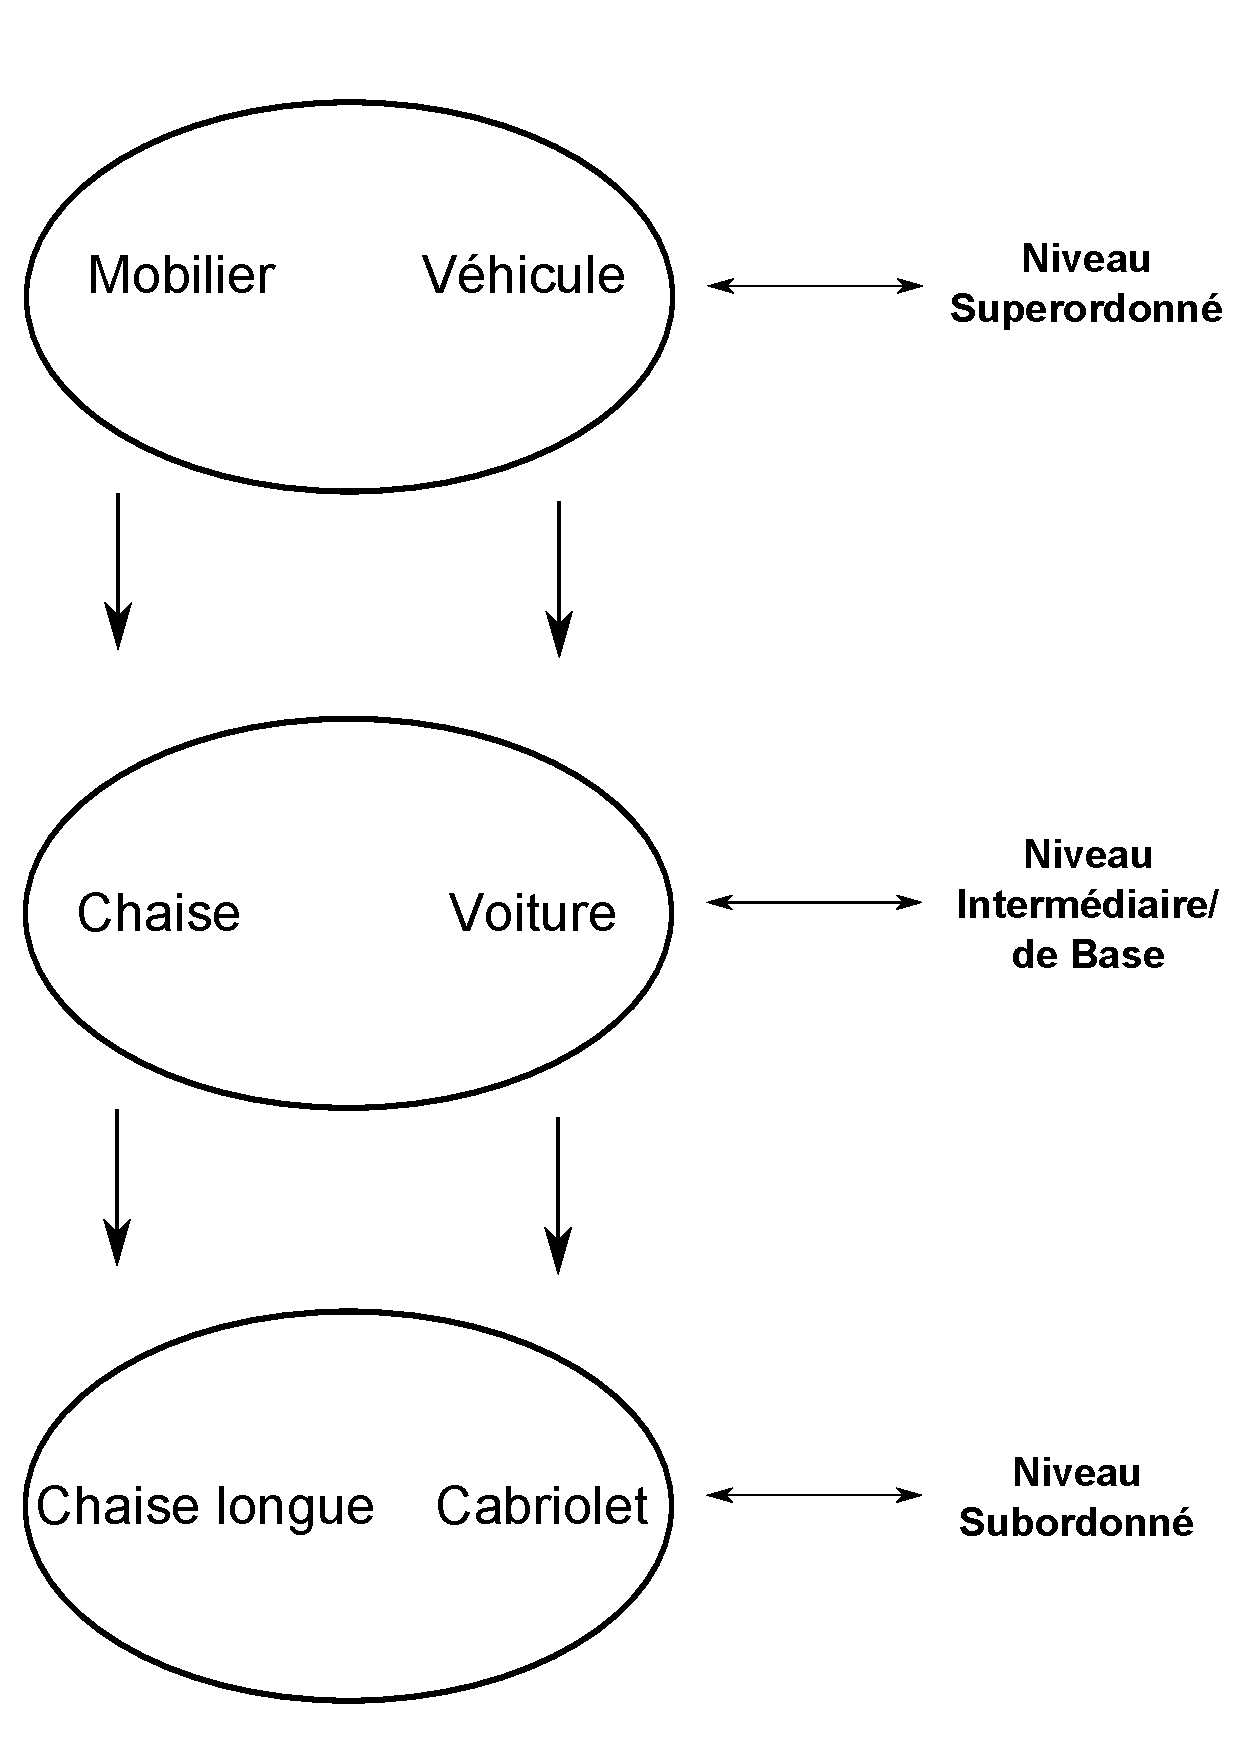
\includegraphics[width=.5\linewidth]{gfx/categorieLVL}
        \caption{Les trois niveaux d'abstraction de l'axe vertical de la structure catégorielle.}\label{fig:categorieLVL}
\end{figure}

Les catégories sont structurées en interne, en référence à un prototype, \ie~l'objet possédant les attributs typiques de celle-ci. L'appartenance d'un objet à une catégorie dépend alors de la ressemblance qu'entretient ce dernier avec le prototype.  Plusieurs proposition ont été faites afin de définir le prototype d'une catégorie: Pour Tversky \citep{tversky1977features}, le membre prototype sont celui dont la somme des similarités avec les autres membres de la catégorie est la plus grande. Pour \citep{rosch1975family}, il s'agit de l'objet possédant le plus de propriétés en commun avec les objets de la catégorie, et le moins de propriétés avec les objets des catégories externes. Dans ce cas, la typicité d'un élément d'une catégorie est donc fonction de son degré d'appartenance à celle-ci, ainsi que de son indépendance vis à vis des autres catégories. En se limitant à l'observation d'attributs vivant dans un espace métrique, \citep{reed1972pattern, rosch1976structural} ont montré que le prototype est un centroid, un objet définit comme étant la moyenne des attributs des objets de la catégories.

Mais il faut bien comprendre que cette théorie prototypique de la catégorisation, bien que se basant sur des faits expérimentaux, est avant tout une vision pratique, un concept qui n'a pas été clairement défini et dont l'implication dans les processus de catégorisation reste floue \citep[p. 36-40]{rosch1978cognition} \citep[p. 49-54]{dubois1991semantique}.

\subsubsection{Implication méthodologique}

L'enjeu des approches catégorielle est de caractériser des catégories mentales soit 1) de paysages sonores, soit de sources sonores. Pour ce faire, on a habituellement recourt à des expériences de description \citep{axelsson2005soundscape,raimbault2005urban,guastavino2006ideal,raimbault2006qualitative}, réalisées via des questionnaires ou interviews, en laboratoire ou dans un cadre \emph{in situ}, ou/et a des expériences de tri \citep{maffiolo_caracterisation_1999,guastavino2007categorization}, pratiquées en laboratoire.

Ces études s'appuient souvent sur des analyses linguistiques et lexicales pratiquées sur les descriptions des sujets, afin d'en faire émerger catégories.

\gl{bien développer sur \citep{dubois1991semantique} afin de justifier l'utilisation du langage}

\subsection{L'approche dimensionnelle}

\subsubsection{Objectif}

\subsubsection{Implication méthodologique}

\subsection{Résultats}

\subsubsection{Catégorisation des sources sonores}

\subsubsection{Catégorisation des environnements sonores}

\subsubsection{Extraction et évaluation des attributs perceptifs}

\gl{bien développer et définir les indicateurs acoustiques et perceptifs, se baser sur \citep{aletta2016soundscape}}
\subsection{Limitations}

%*****************************************
%*****************************************
%*****************************************
%*****************************************
%*****************************************
